
\documentclass[nototal,handout]{beamer}
\mode<presentation>
{
  \usetheme{Madrid}
  \setbeamercovered{transparent}
}

\usepackage{verbatim}
\usepackage{fancyvrb}
\usepackage[english]{babel}
\usepackage[latin1]{inputenc}
\usepackage{times}
\usepackage{tikz}
\usepackage[T1]{fontenc}
\usepackage{graphicx} %sjr added
\graphicspath{{figures/}}
\usepackage{hyperref}

\author{\textsc{Sergio Rey}}
\institute[ASU]{\textbf{GPH 483/598}\\\textbf{Geographic Information Analysis}\\School of Geographical Sciences and Urban Planning\\Arizona State University\\Fall 2010}
\title[Introduction]{Introduction to Geographic Information Analysis}
\subtitle{}
\date[GPH 483/598]{}

% Delete this, if you do not want the table of contents to pop up at
% the beginning of each subsection:
\AtBeginSubsection[]
{
  \begin{frame}<beamer>
    \frametitle{Outline}
    \tableofcontents[currentsection,currentsubsection]
  \end{frame}
}


% If you wish to uncover everything in a step-wise fashion, uncomment
% the following command: 
%\beamerdefaultoverlayspecification{<+->}
\begin{document}
\begin{frame}
  \titlepage
\end{frame}


\begin{frame}{Outline}
  \tableofcontents[pausesections]
\end{frame}



\section{Course Introduction} 

\subsection{Objectives} 

\begin{frame}
	\frametitle{Course Objectives}
 \begin{itemize}
 \item  Introduction to fundamentals of ESDA
 \item  Conceptual background
 \item  Hands-on
 \end{itemize}
 \end{frame} 

\subsection{Content and Structure} 

\begin{frame}
	\frametitle{Components}
 
\begin{block}{Four Sections}
 \begin{itemize}
 \item  Introduction and Background
 \item  Point Patterns
 \item  Spatial Autocorrelation
 \item  Geostatistics
 \end{itemize}
 \end{block} \end{frame} 

\begin{frame}
	\frametitle{Part I: Introduction}
  \begin{center}
    \begin{footnotesize}
\begin{tabular}{|lr|l|l|l|}
\hline
Month & \multicolumn{1}{l|}{Date} & Topic/Readings & Out & Due \\ \hline
Jan & 20 & Introduction to Geographic Information Analysis &  &  \\ 
    &    & GIA 1, GA 1 & &\\
 & 27 & Spatial Data& Exercise 1 &  \\ 
    &    & GIA 2,3, GA 2,4 & &\\
 \hline
\end{tabular}
    \end{footnotesize}
  \end{center}
 \end{frame} 
 
\begin{frame}
	\frametitle{Part II: Point Patterns}
  \begin{center}
    \begin{footnotesize}
\begin{tabular}{|lr|l|l|l|}
\hline
Month & \multicolumn{1}{l|}{Date} & Topic/Readings & Out & Due \\ \hline
Feb & 3 & Point Pattern Basics &Project &  \\ 
    &    & GIA 4 & &\\
 & 10 & Point Pattern Processes & Exercise 2 & Exercise 1 \\ 
    &    & GIA 5 & & \\
     & 17 & Quadrat and Distance Based Methods &  & \\ 
    &    & GA p 211-221 & &\\
 & 24 & Advanced Point Patterns &Data Proposals  & Exercise 2  \\ 
    &    & ASD 7 & &\\
 \hline
\end{tabular}
    \end{footnotesize}
  \end{center}
 \end{frame} 
 

\begin{frame}
	\frametitle{Part III: Lattice Data}
  \begin{center}
    \begin{footnotesize}
\begin{tabular}{|lr|l|l|l|}
\hline
Month & \multicolumn{1}{l|}{Date} & Topic/Readings & Out & Due \\ \hline
Mar & 3 & Lattice Data Basics & Exercise 3 & \\ 
    &    & GIA 7 & &\\
 & 10 & Spatial Weights &  &Data Approval   \\ 
    &    & Anselin and Rey (2010) & &\\
 & 17 & Spring Break &  &  \\ 
 & 24 & Global Autocorrelation & Exercise 4 & Exercise 3 \\ 
    &    &  GA p 222-234 & &\\
 & 31 & Local Autocorrelation &  &  \\ 
    &    & GIA p 203-208, GA p 234-238& &\\
 \hline
\end{tabular}
    \end{footnotesize}
  \end{center}
 \end{frame} 

\begin{frame}
	\frametitle{Part IV: Geostatistical Data}
  \begin{center}
    \begin{footnotesize}
\begin{tabular}{|lr|l|l|l|}
\hline
Month & \multicolumn{1}{l|}{Date} & Topic/Readings & Out & Due \\ \hline
Apr & 7 & Geostatistics Basics &  & Exercise 4 \\ 
    &    & GIA 8& &\\
 & 14 & Variography& Exercise 5 &  \\ 
    &    &  GA 6, ASD p 191-208 & &\\
 & 21 & Kriging &  &  \\ 
    &    & GIA 9, ASD p 208-226& &\\
 & 28 & Future Directions &  & Exercise 5 \\ 
May & 5 &  &  & Projects \\ 
 & 12 &  &  & Presentations \\ \hline
\end{tabular}
    \end{footnotesize}
  \end{center}
 \end{frame} 

\section{Logistics} 

\subsection{Grading} 

\begin{frame}
	\frametitle{Grading}
 
 Grading will be assigned on the following scale: A: 90-100, B:
80-89, C:70-79, D: 60-69, F below 60. There will be no curves and no extra
credit. I will assign +/- on an individual basis. Points are assigned as
follows:

\vspace{.1in}
\begin{center}
\begin{tabular}[h]{|l|rr|}
  \hline
  &\multicolumn{2}{|c|}{Points}\\
  Component&Undergraduate&Graduate\\
  \hline
  Exercises&40&30\\
  Project&40&40\\
  Quizzes&20&20\\
  Presentations& &10\\
  \hline
  TOTAL&100&100\\ \hline
\end{tabular}
\end{center}
\vspace{.1in}

\end{frame} 

\begin{frame}
	\frametitle{Grading 483 vs. 598}
 
\begin{block}{Undergraduate}
  For your project you can either:
 \begin{itemize}
 \item  select your own data
 \item  use data I give you
 \end{itemize}
 \end{block} 
\begin{block}{Graduate}
 \begin{itemize}
 \item  you must select your own data for your project
 \item  present article synopsis
 \item  present final project
 \end{itemize}
 \end{block} 
 \end{frame}

\begin{frame}
	\frametitle{Prerequisites}
  All participants are expected to have  working knowledge of spatial
  analysis concepts and to be familiar with multivariate statistics. No
  extensive GIS background beyond ArcGIS basics is needed.
 \end{frame} 

\begin{frame}
	\frametitle{Course Organization}

The course will meet in CoorL 1-18. The first part of each
weekly meeting will focus on background and theoretical material related to
the particular type of spatial data analysis. Following a short break, the
attention will shift to introduce various software packages for the analysis
of spatial data.
 \end{frame} 

 \begin{frame}
   \frametitle{Ground Rules}
   \begin{block}{Classroom etiquette}
      To ensure a productive learning environment, all
participants are expected to abide by the following rules:
\begin{itemize}
  \item Because we are meeting in a computer laboratory
food is strictly forbidden in the class meetings.
\item Use of the classroom computers should only be in support of the course.
  Extracurricular use (i.e., browsing non-course materials, using  social networks, checking
  email, chat sessions, etc) during class meetings is disruptive for your colleagues and
  disrespectful. Individuals violating this rule will be asked to leave for
  that course session.
\end{itemize}

    \end{block}
  \end{frame}

\subsection{Readings} 

\begin{frame}
\frametitle{Readings}
\begin{block}{Textbooks}
Assigned readings are listed in the schedule and are to be
done prior to class meeting. The majority of these are taken from the
following texts:
\begin{description}
  \item[GIA] David O'Sullivan and
David J. Unwin (2006) \emph{Geographic Information Analysis}, Wiley: Hoboken
  \item[GA] 
Michael de Smith, Michael F. Goodchild, and Paul A. Longley (2007) \emph{Geospatial
Analysis}, Winchelsea Press: Leicester\\
\item[ASD] Roger S. Bivand, Edzer J. Pebesma and Virgilio G\'omez-Rubio (2008)
  \emph{Applied Spatial Data Analysis with R}, Springer: New York.
\end{description}

Additional readings will be assigned by topic.


\end{block}

\end{frame}

\subsection{Software} 

\begin{frame}
	\frametitle{Software}
  \centering
 \begin{tabular}{l}
  GeoDa\\
    \url{http://geodacenter.asu.edu/software/downloads}
    \\ \hline
   R\\
    \url{http://cran.r-project.org/}
    \\
    \hline
   STARS
   \\
    \url{http://regionalanalysislab.org/index.php/Main/STARS}	
    \\
    \hline
 \end{tabular}
 \end{frame} 


\section{GIS and Spatial Analysis} 

\subsection{Big Picture} 

\begin{frame}
	\frametitle{GIS Then}
 \begin{center}
 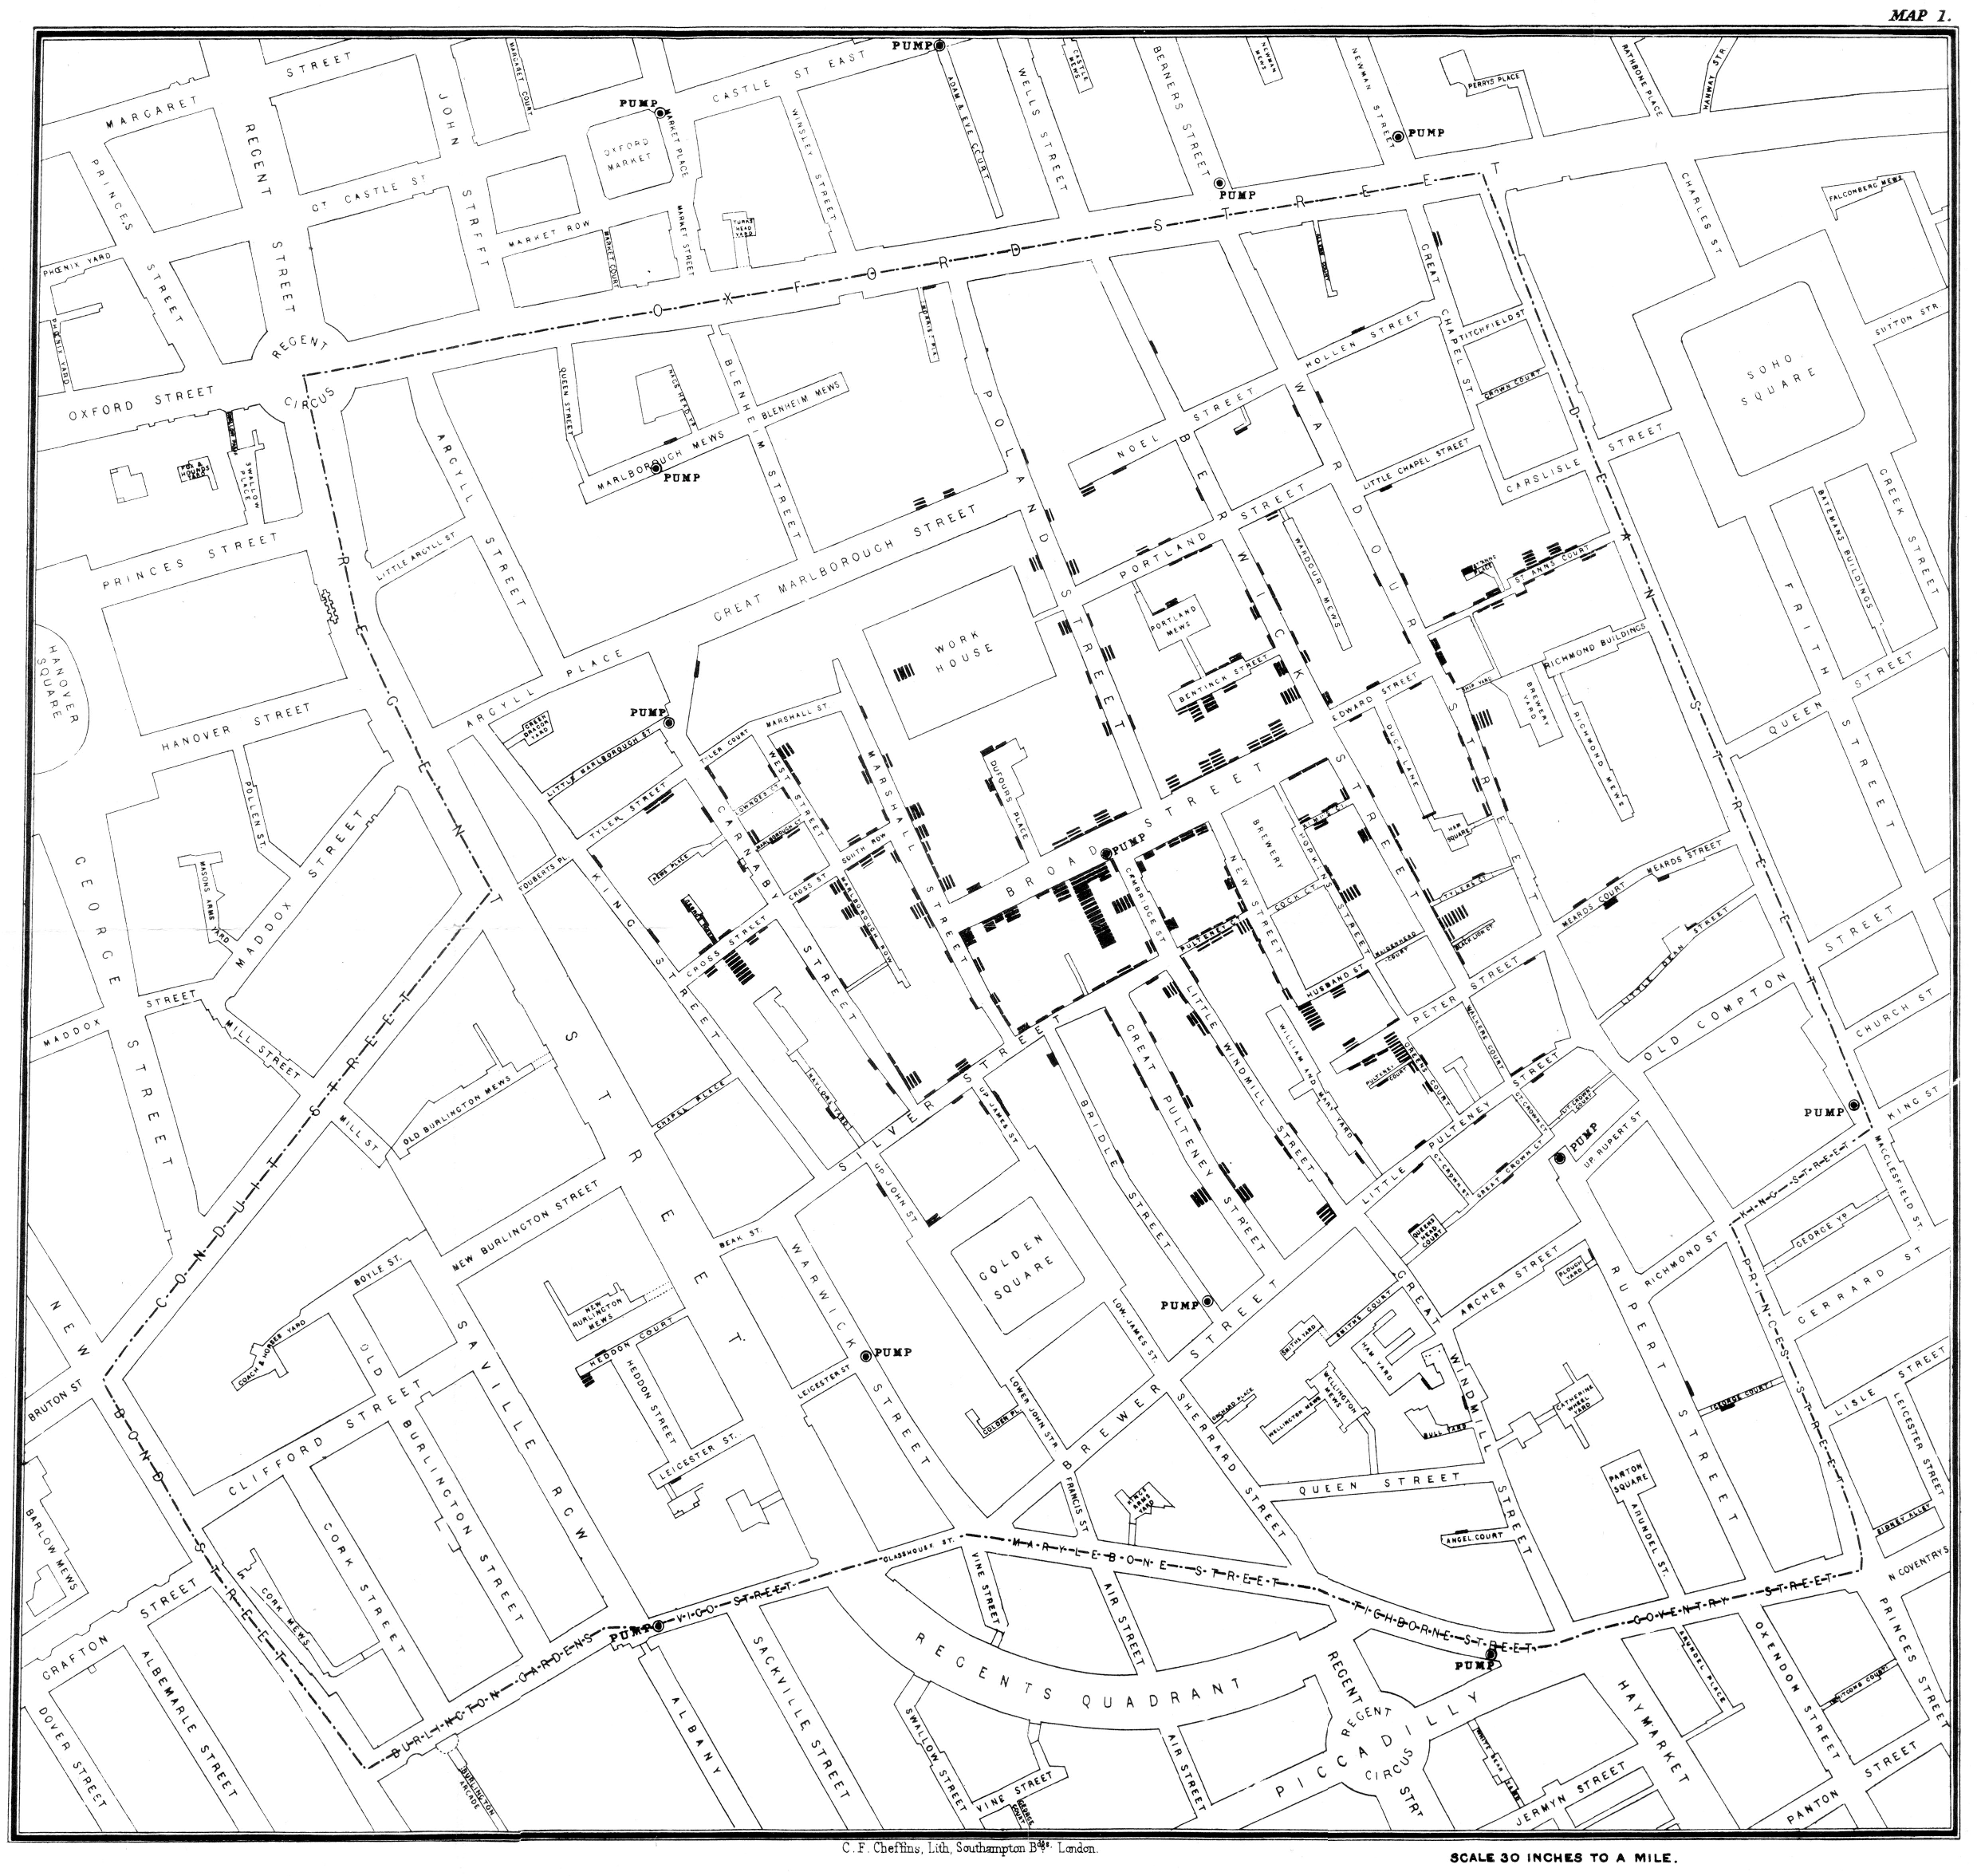
\includegraphics[width=.85\linewidth]{snowmap1.pdf}
  \end{center}
 \end{frame} 

\begin{frame}
	\frametitle{GIS Then}
 \begin{center}
 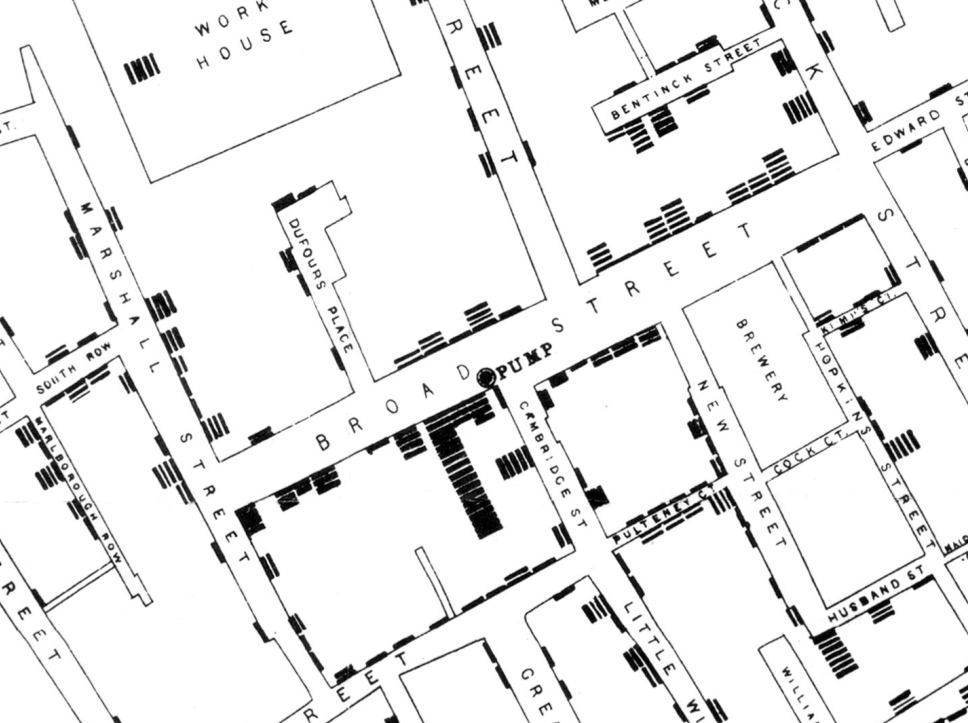
\includegraphics[width=.85\linewidth]{snowmap3.png}
  \end{center}
 \end{frame} 

\begin{frame}
	\frametitle{GIS Now}
 \begin{center}
 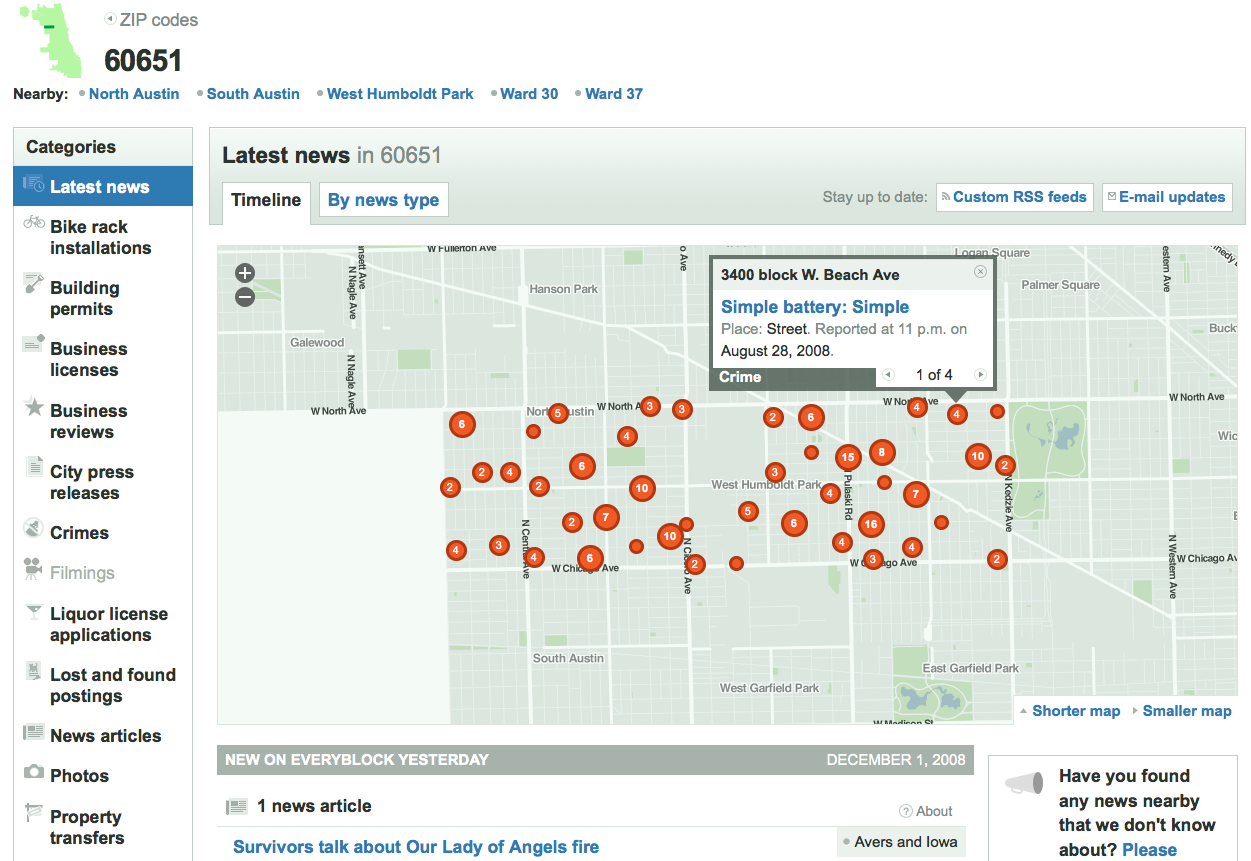
\includegraphics[width=.85\linewidth]{crimemap.png}
  \end{center}
 \end{frame} 

\begin{frame}
	\frametitle{GIS Functions}
 
\begin{block}{Anselin-Getis (1992) Taxonomy}
 \begin{itemize}
 \item  Input
 \item  Storage
 \item  \alert{Analysis}
 \item  Output
 \end{itemize}
  Many other taxonomies
 \end{block} \end{frame} 

\begin{frame}
	\frametitle{GIScience}
 
\begin{block}{Goodchild (1992)}
 \begin{itemize}
 \item  cross-disciplinary
 \item  \alert{central} role for spatial analysis
 \item  scientific \alert{glue}
 \end{itemize}
 \end{block} \end{frame} 

\subsection{What is Spatial Analysis?} 

\begin{frame}
	\frametitle{What is Spatial Analysis?}
 
\begin{block}{From Data to Information}
 \begin{itemize}
 \item  \alert{Beyond} mapping
 \item  \alert{added value}
 \item  transformations, manipulations and application of analytical methods to spatial (geographic data)
 \end{itemize}
 \end{block} \end{frame} 

\begin{frame}
	\frametitle{Locational Invariance}
 
\begin{block}{How Insights  Change with location}
 \begin{itemize}
 \item  spatial analysis is \alert{not} locationally invariant
 \item  the results change when the locations of the study objects change
 \item  \alert{where} matters
 \end{itemize}
 \end{block} \end{frame} 

\begin{frame}
	\frametitle{State Income Distributions 1929}
 \begin{center}
 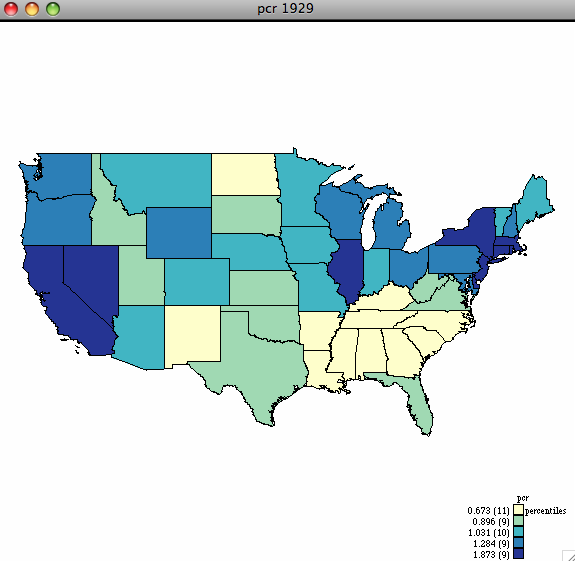
\includegraphics[width=.65\linewidth]{income29.png}
  \end{center}
 \end{frame} 

\begin{frame}
	\frametitle{State Income Distributions 1929}
 \begin{center}
 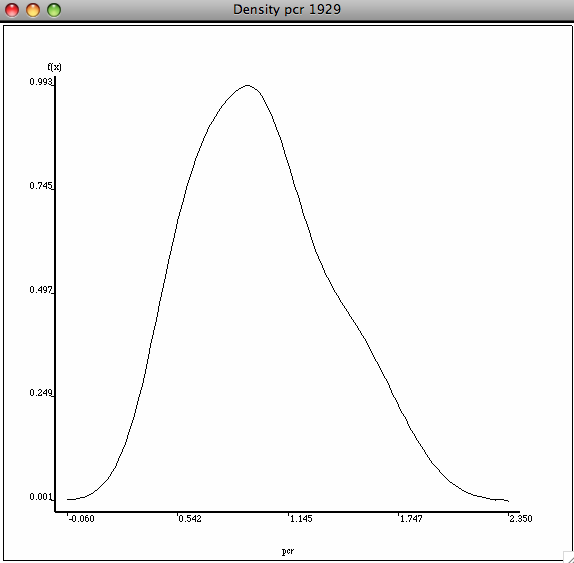
\includegraphics[width=.65\linewidth]{density29.png}
  \end{center}
 \end{frame} 

\begin{frame}
	\frametitle{Randomized Income Distribution 1929}
 \begin{center}
 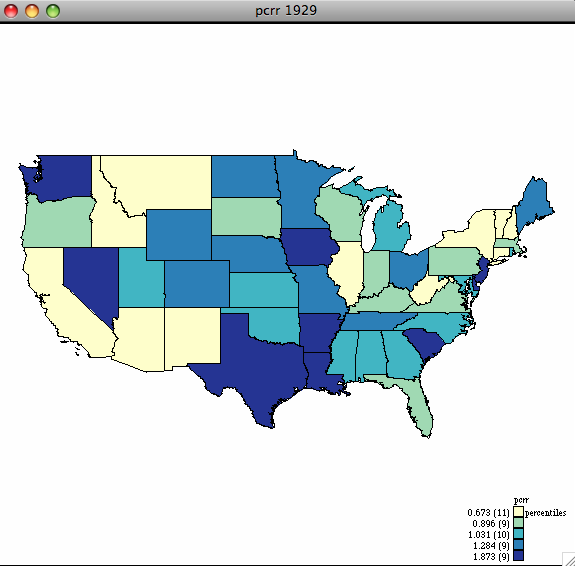
\includegraphics[width=.65\linewidth]{income29random.png}
  \end{center}
 \end{frame} 

\begin{frame}
	\frametitle{Randomized Income Density 1929}
 \begin{center}
 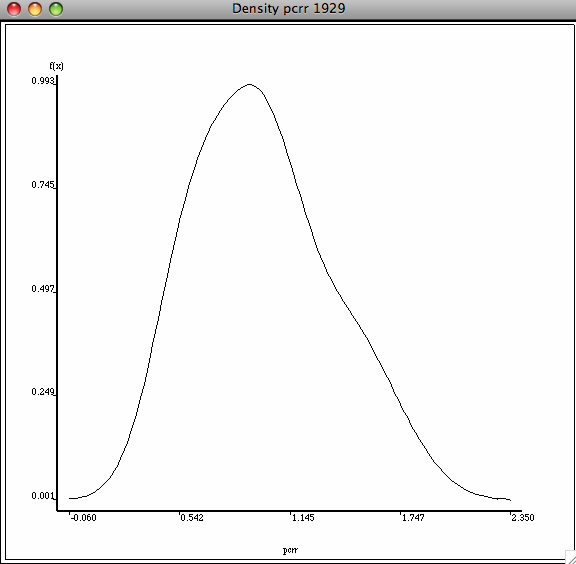
\includegraphics[width=.65\linewidth]{density29random.png}
  \end{center}
 \end{frame} 

\begin{frame}
	\frametitle{Locational Invariance}
 \begin{figure}[ht]
  \begin{minipage}[b]{0.4\linewidth}
  \centering
  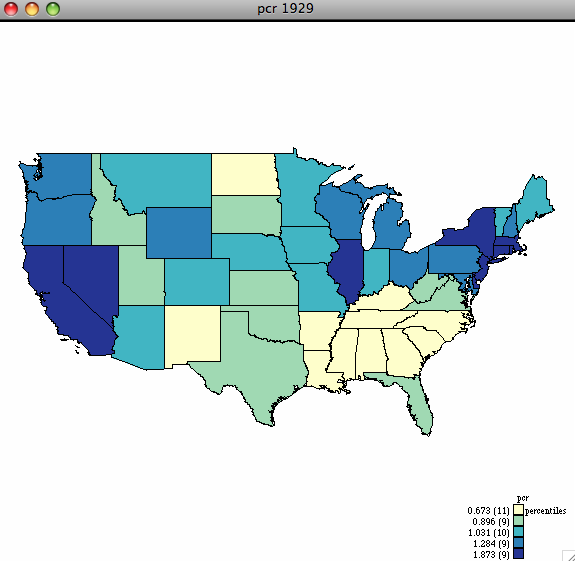
\includegraphics[scale=0.20]{income29.png}
  \end{minipage}
  \begin{minipage}[b]{0.4\linewidth}
  \centering
  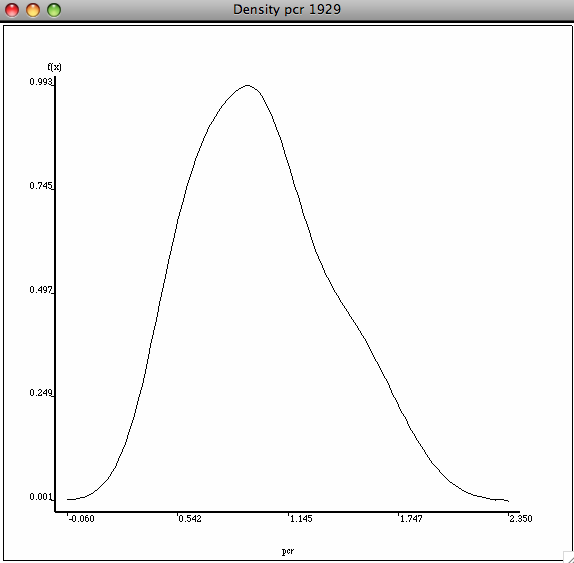
\includegraphics[scale=0.20]{density29.png}
  \end{minipage}
 \begin{minipage}[b]{0.4\linewidth}
  \centering
  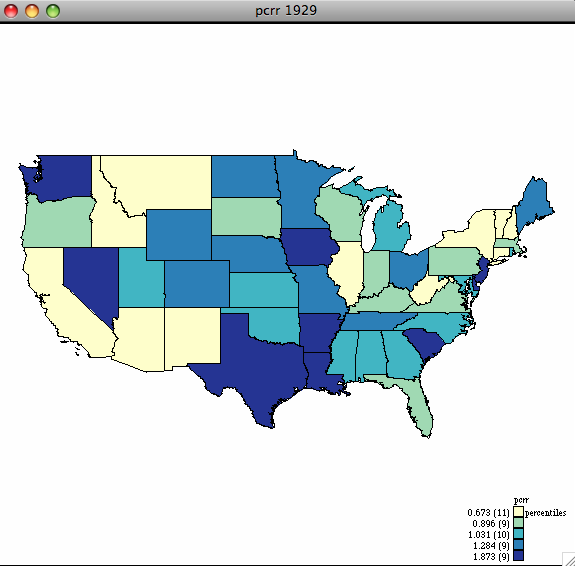
\includegraphics[scale=0.20]{income29random.png}
  \end{minipage}
 \begin{minipage}[b]{0.4\linewidth}
  \centering
  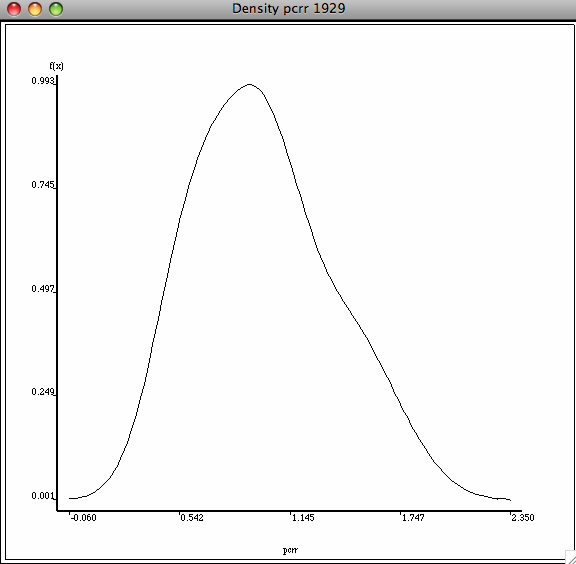
\includegraphics[scale=0.20]{density29random.png}
  \end{minipage}
  \end{figure}
 \end{frame} 

\begin{frame}
	\frametitle{Spatial Autocorrelation Income 1929}
 \begin{center}
 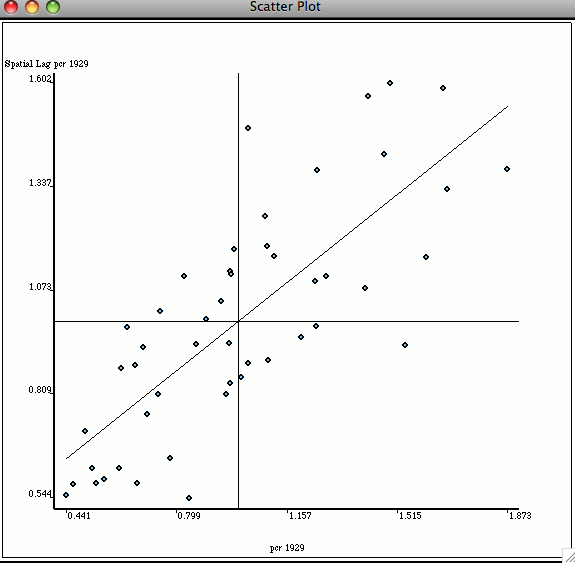
\includegraphics[width=.65\linewidth]{moran29.png}
  \end{center}
 \end{frame} 

\begin{frame}
	\frametitle{Spatial Autocorrelation Randomized Income 1929}
 \begin{center}
 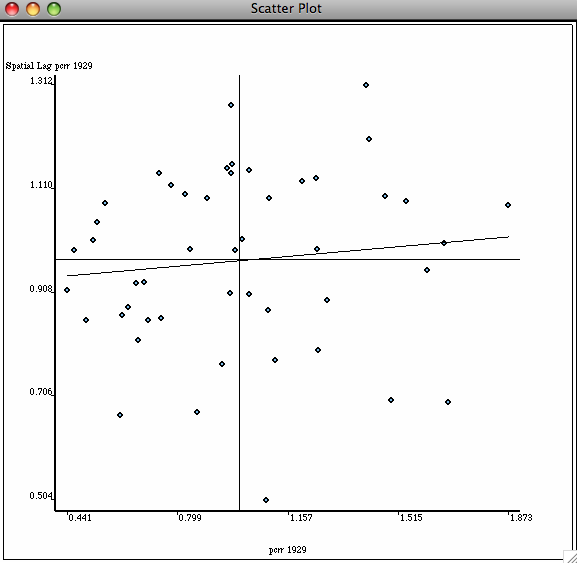
\includegraphics[width=.65\linewidth]{moran29random.png}
  \end{center}
 \end{frame} 

\begin{frame}
	\frametitle{Locational Invariance}
 \begin{figure}[ht]
  \begin{minipage}[b]{0.4\linewidth}
  \centering
  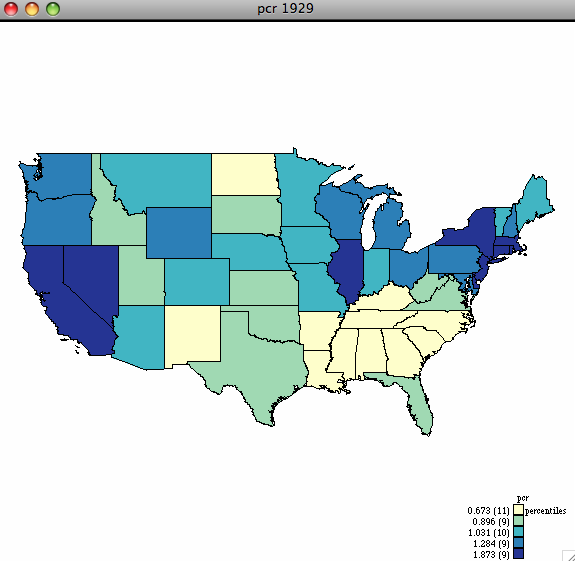
\includegraphics[scale=0.20]{income29.png}
  \end{minipage}
  \begin{minipage}[b]{0.4\linewidth}
  \centering
  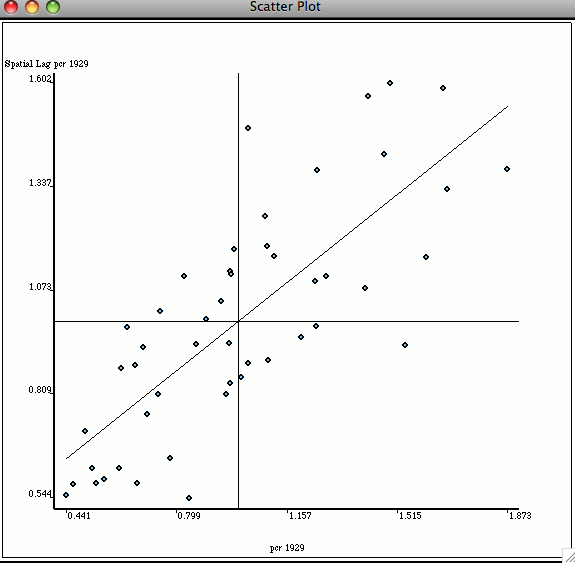
\includegraphics[scale=0.20]{moran29.png}
  \end{minipage}
 \begin{minipage}[b]{0.4\linewidth}
  \centering
  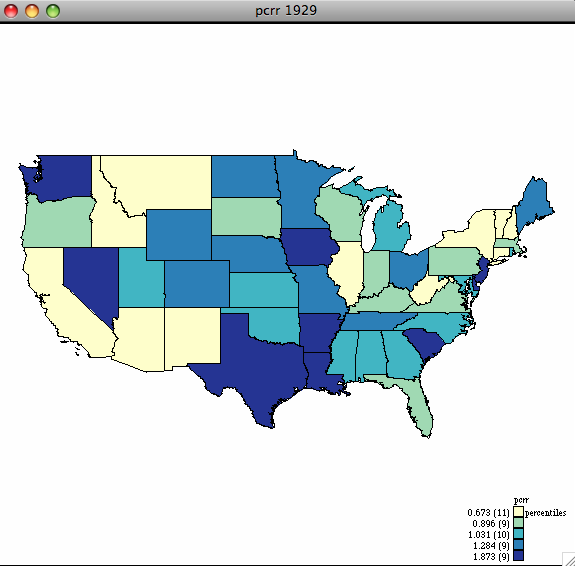
\includegraphics[scale=0.20]{income29random.png}
  \end{minipage}
 \begin{minipage}[b]{0.4\linewidth}
  \centering
  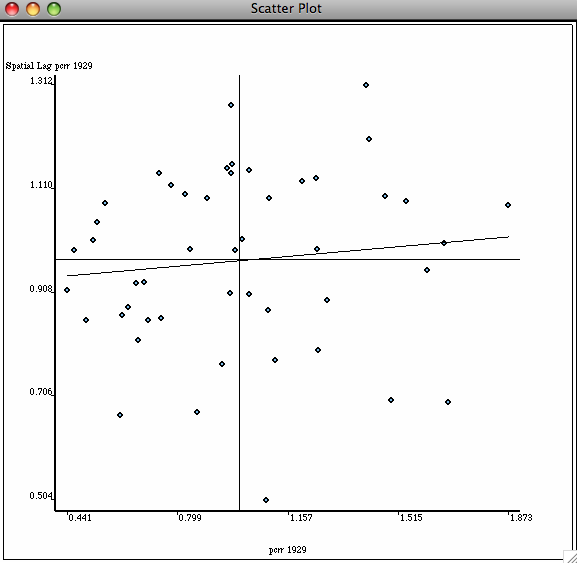
\includegraphics[scale=0.20]{moran29random.png}
  \end{minipage}
  \end{figure}
 \end{frame} 

\begin{frame}
	\frametitle{Components of Spatial Analysis}
 
\begin{block}{Mapping and Geovisualization}
  \alert{showing} interesting patterns
 \end{block} 
\begin{block}{Exploratory Spatial Data Analysis}
  \alert{discovering} interesting patterns
 \end{block} 
\begin{block}{Spatial Modeling}
  \alert{explaining} interesting patterns
 \end{block} \end{frame} 

\begin{frame}
	\frametitle{Summary: Spatial Analysis}
 
\begin{block}{Beyond Mapping}
  Central role for \alert{analysis}
 \end{block} 
\begin{block}{Distinguished by Locational Variance}
  \alert{Location} matters
 \end{block} 
\begin{block}{Components}
  Showing, discovering, explaining
 \end{block} \end{frame} 


\section{EDA and ESDA} 

\subsection{Exploratory Data Analysis (EDA)} 

\begin{frame}
	\frametitle{What is EDA?}
 
\begin{block}{Philosophy}
  EDA is an approach, not simply a set of techniques, but an
  attitude/philosophy about how a data analysis should be carried
  out.
 
 Postpones the usual assumptions about what kind of model the data follow
 \end{block} 
\begin{block}{Origins}
  Tukey, J. (1977) \emph{Exploratory Data Analysis}. Addison,
  Wesely
 \end{block} \end{frame} 

\begin{frame}
	\frametitle{Components}
 
\begin{block}{Set of techniques to}
 \begin{itemize}
 \item  maximize insight into a data set
 \item  uncover underlying structures
 \item  extract important variables
 \item  detect outliers and anonalies
 \item  test underlying assumptions
 \item  suggest hypotheses
 \item  develop parsimonious models
 \end{itemize}
 \end{block} \end{frame} 

\begin{frame}
	\frametitle{EDA Techniqes}
 
\begin{block}{Statistical Graphics}
 \begin{itemize}
 \item  EDA relies heavily on statistical graphics
 \item  EDA is not identical to statistical graphics
 \item  Graphics support pattern recognition and open-minded exploration
 \item  Interactive graphcs push this even further
 \end{itemize}
 \end{block} 
\begin{block}{Quantitiatve Methods}
  Although heavily graphic in orientation, there are also a number
  of numerical techniques in EDA.
 \end{block} \end{frame} 

\begin{frame}
	\frametitle{EDA Versus Confirmatory Analysis}
 
\begin{block}{Confirmatory Analysis (e.g. regression)}
  Problem $\rightarrow$ Theory $\rightarrow$ Model $\rightarrow$ Data $\rightarrow$ Conclusion
 \end{block} 
\begin{block}{Exploratory Analysis}
  Problem $\rightarrow$ Data $\rightarrow$ Analysis $\rightarrow$ Model
 \end{block} \end{frame} 

\subsection{Exploratory Spatial Data Analysis (ESDA)} 

\begin{frame}
	\frametitle{What is ESDA?}
 
\begin{block}{Definitions}
 \begin{itemize}
 \item  Type of EDA
 \item  Extended to include spatial attributes of the data
 \end{itemize}
 \end{block} 
\begin{block}{Crossfertilization}
 \begin{itemize}
 \item  Applying classic EDA to spatial data
 \item  Developing new EDA methods for spatial data
 \item  Interactions between EDA and ESDA
 \end{itemize}
 \end{block} \end{frame} 

\begin{frame}
	\frametitle{How does ESDA fit in spatial analysis?}
 
\begin{block}{Spatial Modeling?}
 \begin{itemize}
 \item  Modeling based on assumptionss
 \item  ESDA largely model free
 \item  Matter of degree (e.g., clustering)
 \end{itemize}
 \end{block} 
\begin{block}{Mapping?}
 \begin{itemize}
 \item  Maps play a critical role in ESDA
 \item  Does a map = ESDA?
 \item  No. ESDA = map, manipulation + visualization
 \end{itemize}
 \end{block} \end{frame} 

\subsection{Geovisualization} 

\begin{frame}
	\frametitle{Geovisualization}
 
\begin{block}{Beyond Mapping}
 \begin{itemize}
 \item  Combing map and scientific visualization methods
 \item  Exploit human pattern recognition capabilities
 \end{itemize}
 \end{block} 
\begin{block}{Statistical Maps}
 \begin{itemize}
 \item  innovative map devices
 \end{itemize}
 \end{block} \end{frame} 

\begin{frame}
	\frametitle{Mapping Issues}
 
\begin{block}{How to Lie with Maps}
 \begin{itemize}
 \item  Monmonnier (1996)
 \item  many design issues
 \item  projects
 \item  human perception can be tricked
 \end{itemize}
 \end{block} \end{frame} 

\begin{frame}
	\frametitle{Visual Analytics}
 
\begin{block}{The Science of Analytical Reasoning Facilitated by Interactive Visual Interfaces}
 \begin{itemize}
 \item  NVAC 2005
 \item  science of analytical reasoning
 \item  visual representation and interaction
 \item  data representation and transformations
 \item  production, presentation and dissemination
 \end{itemize}
 \end{block} \end{frame} 

\begin{frame}
	\frametitle{Visual Analysis}
 
\begin{block}{Tools}
 \begin{itemize}
 \item  synthesize inforation
 \item  derive insights
 \item  detect the expected and discover the unexpected
 \item  understandable assessments
 \item  communicate effectively
 \item  focused on policy actions
 \end{itemize}
 \end{block} \end{frame} 

\begin{frame}
	\frametitle{Visual Explanations}
 
\begin{block}{Tufte (1997)}
  Reasoning about Evidence and Design of Graphics
 \begin{itemize}
 \item  documenting sources (metadata)
 \item  appropriate comparisons
 \item  quantify and show cause and effect
 \item  multivariate nature of analytic problems
 \item  evaluate alternative explanations
 \end{itemize}
 \end{block} \end{frame} 

\begin{frame}
	\frametitle{Choropleth Map}
 
\begin{block}{Map Counterpart of Histogram}
 \begin{itemize}
 \item  values for discrete spatial uits
 \item  choro from  choros (region) NOT chloro
 \end{itemize}
 \end{block} 
\begin{block}{Discrete Approximations}
 \begin{itemize}
 \item  intervals
 \item  continuous shading
 \end{itemize}
 \end{block} \end{frame} 

\begin{frame}
	\frametitle{Map Design Issues}
 
\begin{block}{Choice of Intervals}
 \begin{itemize}
 \item  cut points: equal interval, natural breaks
 \item  statistical criteria: equal area (quantile)
 \end{itemize}
 \end{block} 
\begin{block}{Choice of Colors}
 \begin{itemize}
 \item  important for perception of pattern
 \end{itemize}
 \end{block} \end{frame} 

\begin{frame}
	\frametitle{Income Quintiles}
 \begin{center}
 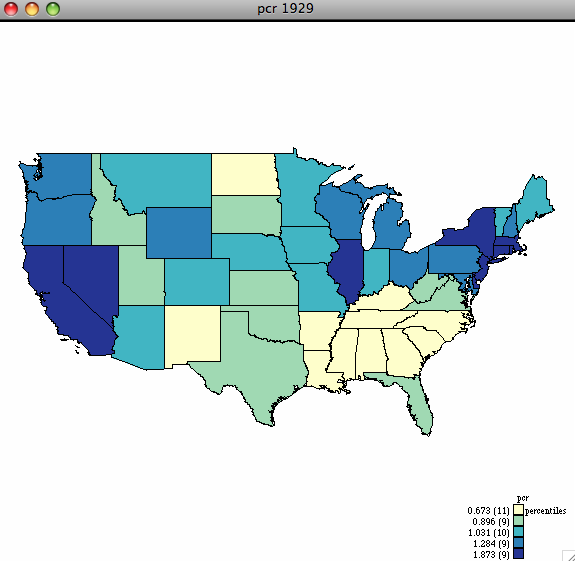
\includegraphics[width=.65\linewidth]{income29.png}
  \end{center}
 \end{frame} 

\begin{frame}
	\frametitle{Outlier Map}
 
\begin{block}{Box Map}
 \begin{itemize}
 \item  Special Quartile Map
 \item  Outliers Highighlited
 \begin{itemize}
 \item  same  criteria as a box plot
 \item  outliers added as extra categories
 \item  six instead of four categories
 \end{itemize}
 \item  Both Magnitude and Location
 \end{itemize}
 \end{block} \end{frame} 

\begin{frame}
	\frametitle{Box Map}
 \begin{center}
 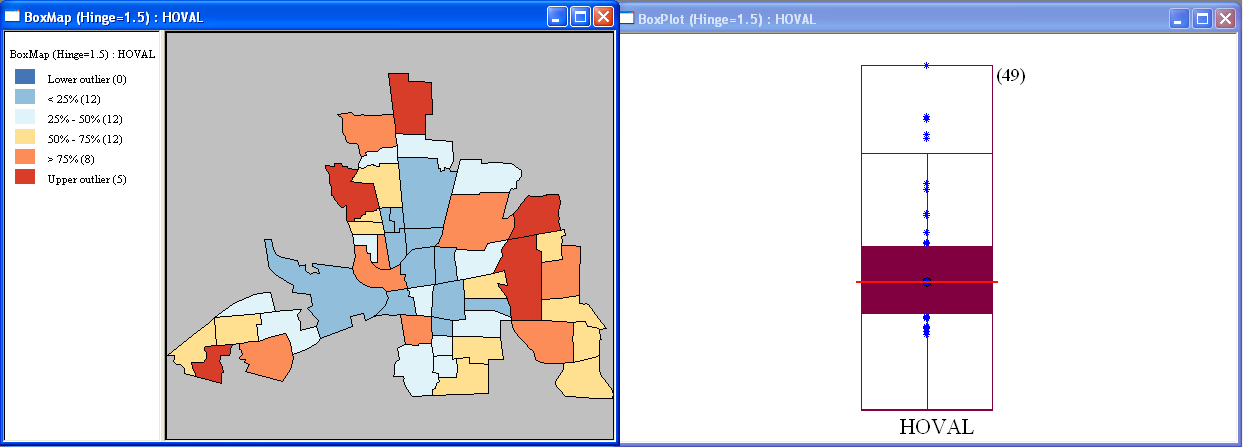
\includegraphics[width=.85\linewidth]{boxmapgeoda.png}
  \end{center}
 \end{frame} 

\begin{frame}
	\frametitle{Special Maps}
 \begin{itemize}
 \item  Cartogram
 \item  Conditional Maps
 \item  Map Animation
 \end{itemize}
 \end{frame} 

\begin{frame}
	\frametitle{Cartogram}
 
\begin{block}{Objectives}
 \begin{itemize}
 \item  Correct for  misleading effect of area
 \begin{itemize}
 \item  larger area units  draw attention
 \item  change layout to reflect size other than area
 \end{itemize}
 \item  Respect topology
 \end{itemize}
 \end{block} 
\begin{block}{Circular Cartogram}
 \begin{itemize}
 \item  variable maps to area/radius of circle
 \end{itemize}
 \end{block} \end{frame} 

\begin{frame}
	\frametitle{Cartogram}
 \begin{center}
 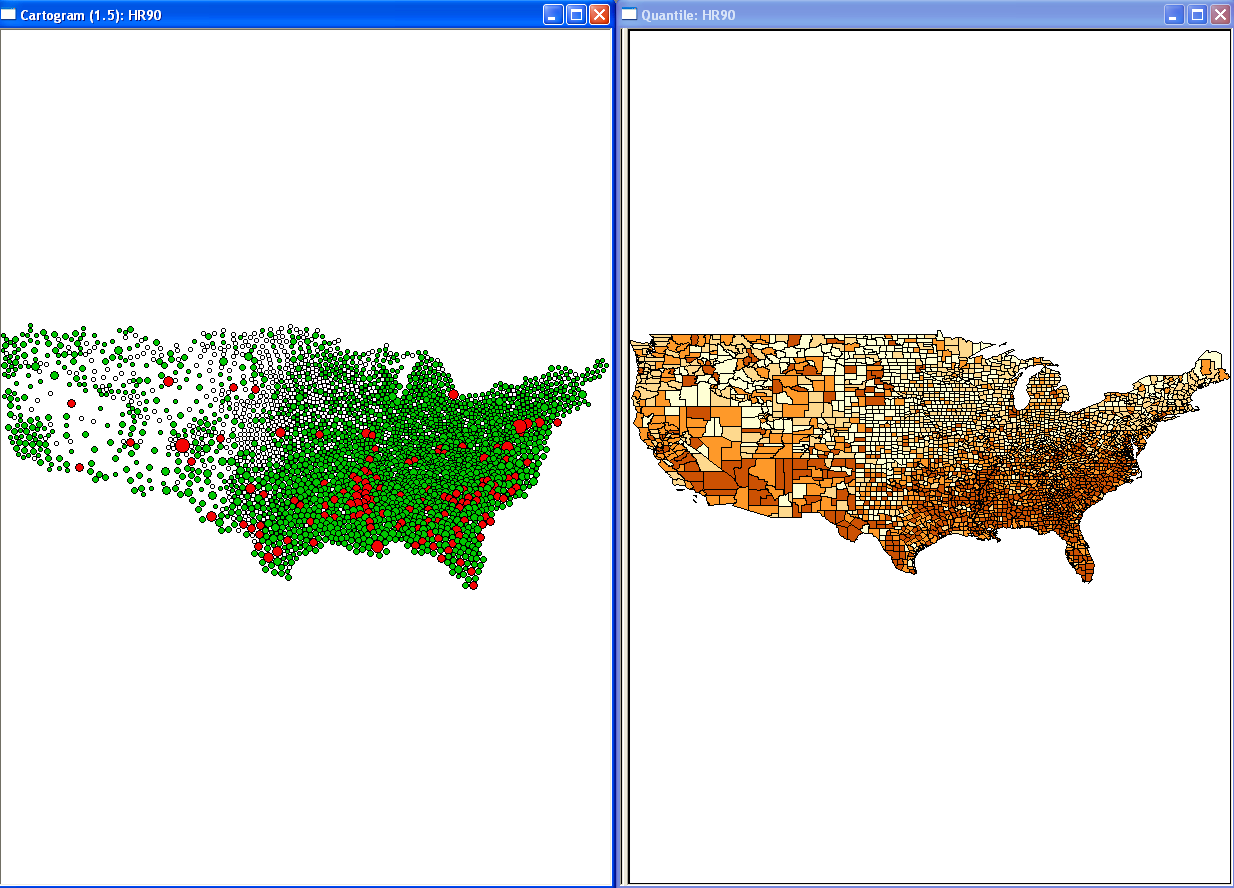
\includegraphics[width=.85\linewidth]{cartogram.png}
  \end{center}
 \end{frame} 

\begin{frame}
	\frametitle{Conditional Maps}
 
\begin{block}{Conditional Choropleth Map (Carr)}
 \begin{itemize}
 \item  Special case of conditional plots
 \item  trellis graphs	
 \end{itemize}
 \end{block} 
\begin{block}{Conditioning}
 \begin{itemize}
 \item  along two dimensions (variables)
 \item  micromap matrix
 \item  choropleth map on dependent variable
 \end{itemize}
 \end{block} \end{frame} 

\begin{frame}
	\frametitle{Conditional Choropleth: Univariate Conditioning}
 \begin{center}
 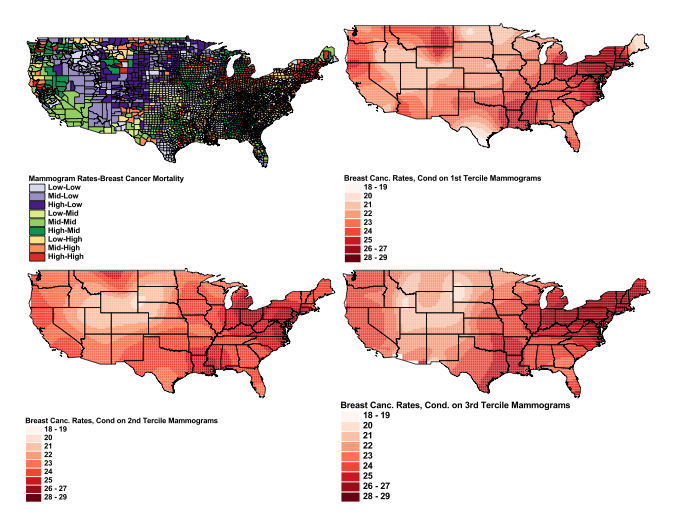
\includegraphics[width=.85\linewidth]{conditionalchoropleth.png}
  \end{center}
 \end{frame} 

\begin{frame}
	\frametitle{Conditional Choropleth: Bivariate Conditioning}
 \begin{center}
 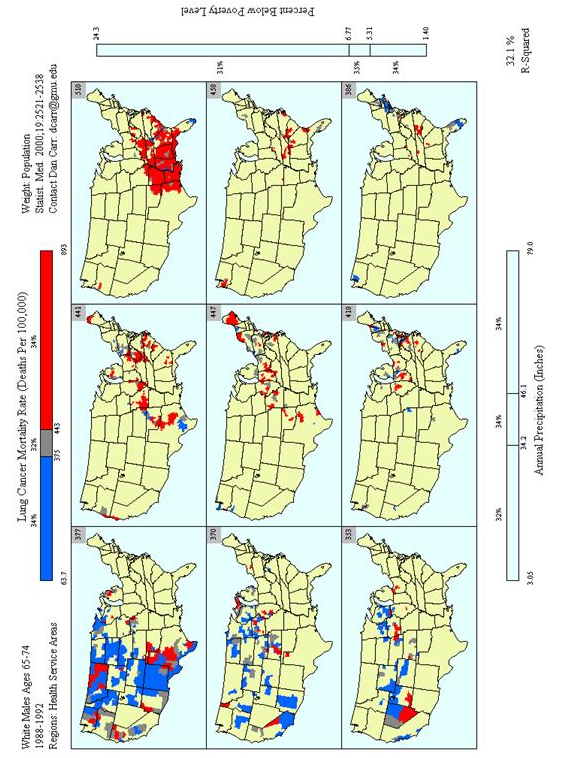
\includegraphics[angle=270,width=.85\linewidth]{conditionalchoropleth1.png}
  \end{center}
 \end{frame} 

\begin{frame}
	\frametitle{Map Animation}
 
\begin{block}{Map Movie}
 \begin{itemize}
 \item  location highlighted in turn
 \item  from low value to high value
 \end{itemize}
 \end{block} 
\begin{block}{Looking for pattern}
 \begin{itemize}
 \item  spatial  heterogeneity
 \item  systematic movements/locations
 \end{itemize}
 \end{block} \end{frame} 

\begin{frame}
	\frametitle{Map Animation}
 Demo
 \end{frame} 

\begin{frame}
	\frametitle{Interactive Graphics}
 
\begin{block}{Interactive View Manipulation}
 \begin{itemize}
 \item  the analyst interacts with the data
 \item  dynamic graphics
 \item  no longer passive
 \end{itemize}
 \end{block} \end{frame} 

\begin{frame}
	\frametitle{Linking and Brushing}
 
\begin{block}{Linking}
 \begin{itemize}
 \item  selection in one graph is simultaneously selected in all
 \end{itemize}
    graphs
 \end{block} 
\begin{block}{Brushing}
 \begin{itemize}
 \item  changing the selection set is dynamically updated in all graphs and maps
 \end{itemize}
 \end{block} \end{frame} 

\begin{frame}
	\frametitle{Linking}
 \begin{center}
 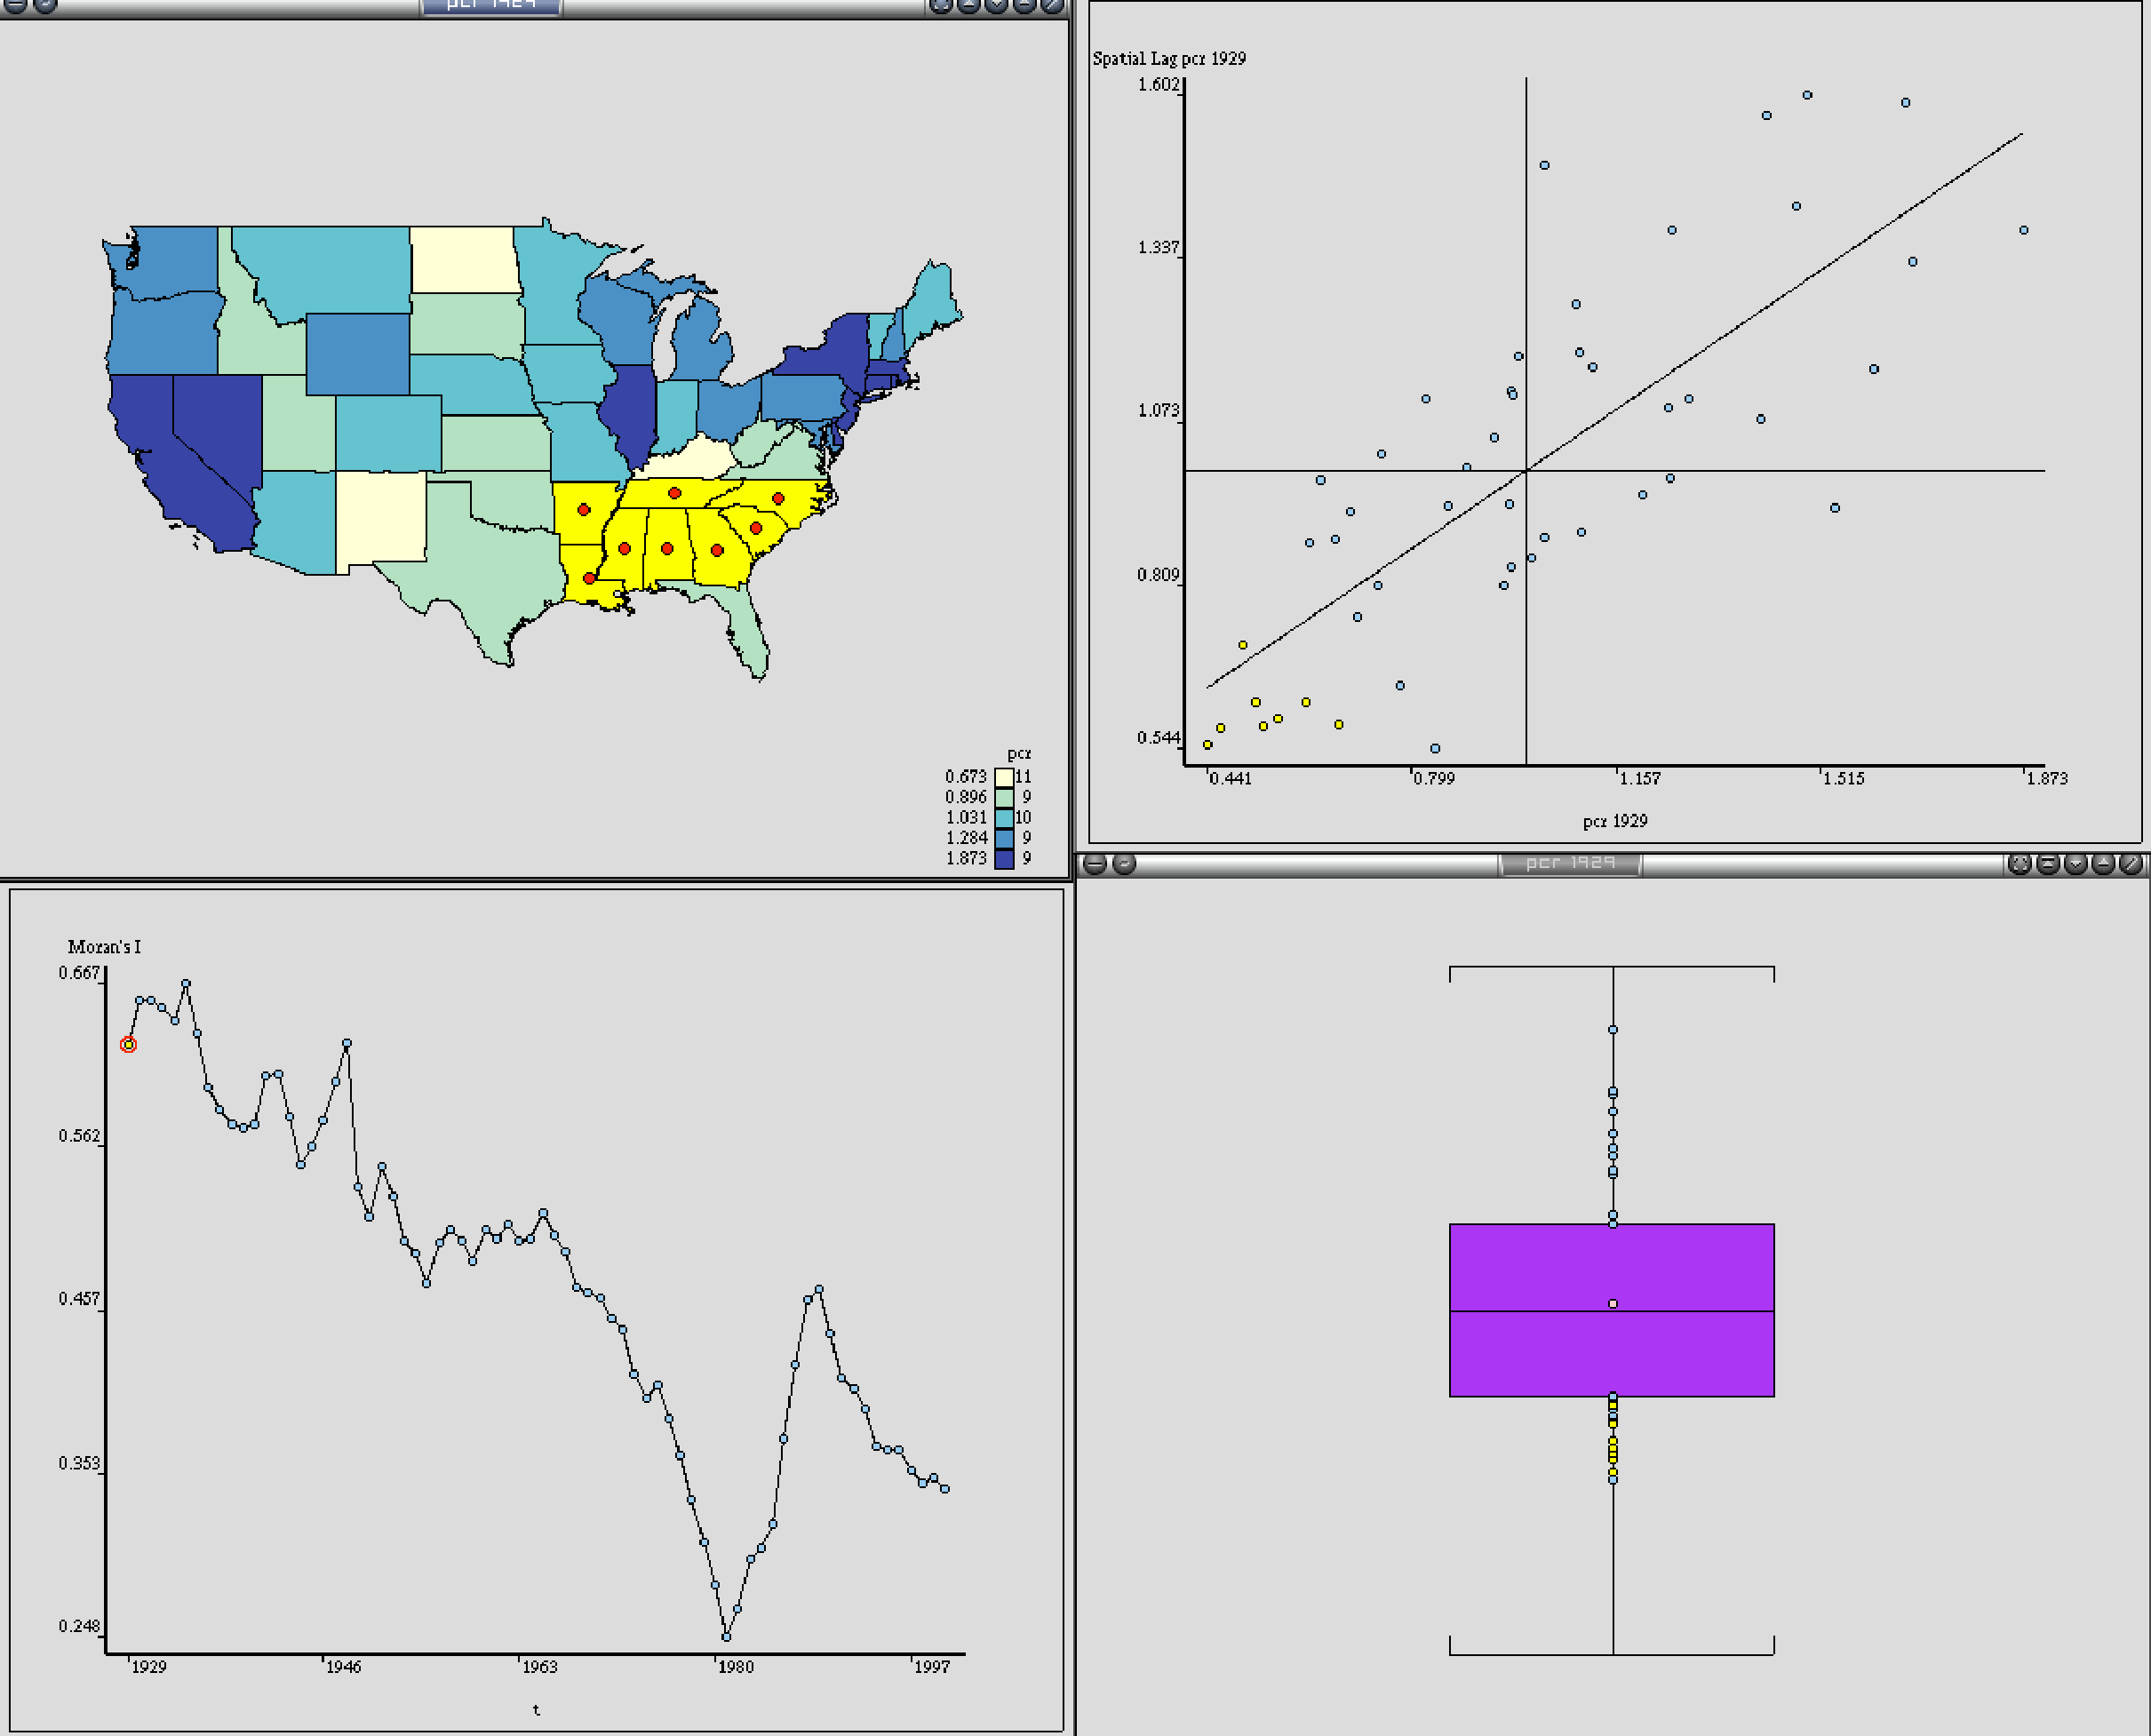
\includegraphics[width=.85\linewidth]{linking.pdf}
  \end{center}
 \end{frame} 

\begin{frame}
	\frametitle{Brushing a  Scatter Plot}
 \begin{center}
 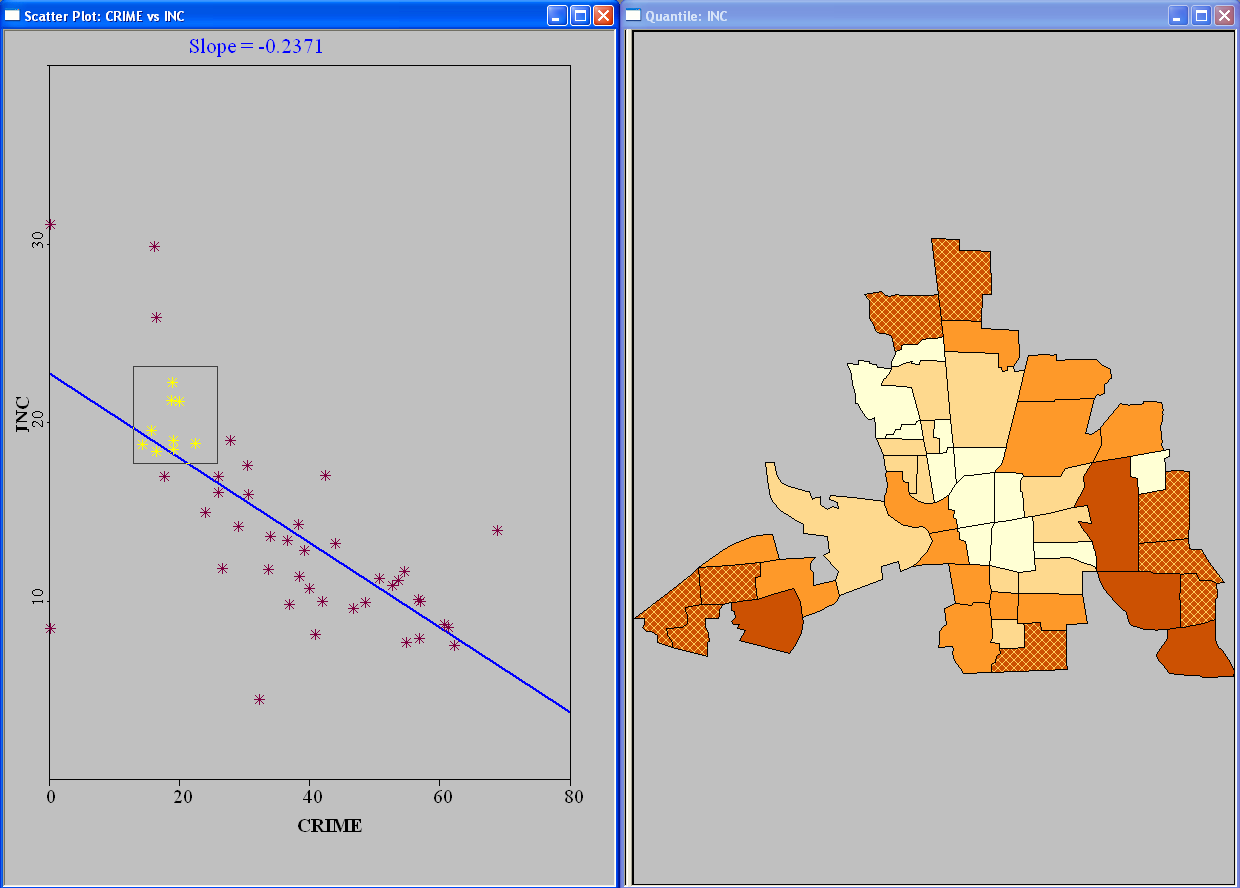
\includegraphics[width=.85\linewidth]{brushspgeoda.png}
  \end{center}
 \end{frame} 

\begin{frame}
	\frametitle{Brushing a  Map}
 \begin{center}
 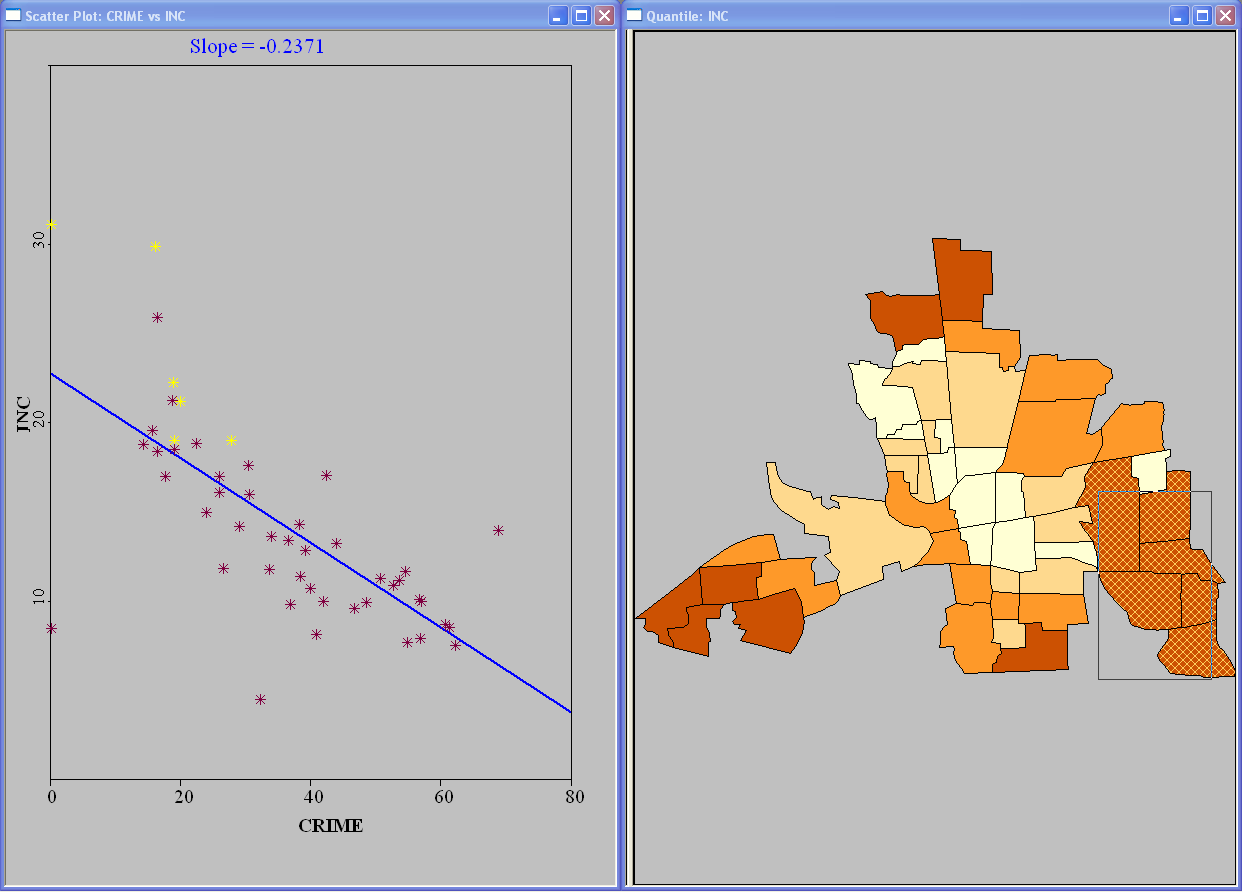
\includegraphics[width=.85\linewidth]{brushmapgeoda.png}
  \end{center}
 \end{frame} 

\begin{frame}
	\frametitle{Multivariate EDA}
 \begin{itemize}
 \item  Scatter Plot Matrix
 \item  Parallel Coordinate Plot
 \item  3-D Scatter Plot
 \end{itemize}
 \end{frame} 

\begin{frame}
	\frametitle{Scatter Plot Matrix}
 \begin{center}
 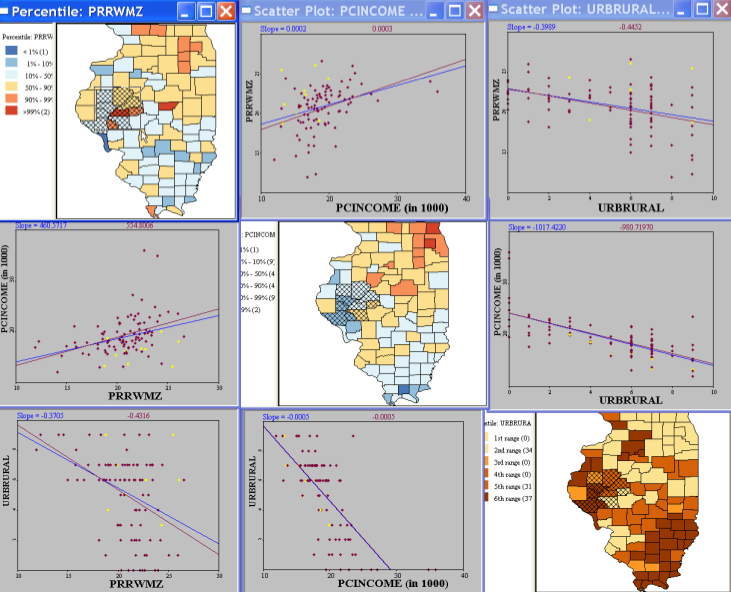
\includegraphics[width=.85\linewidth]{spmatrix.png}
  \end{center}
 \end{frame} 

\begin{frame}
	\frametitle{Brushing a  Parallel Coordinate Plot}
 \begin{center}
 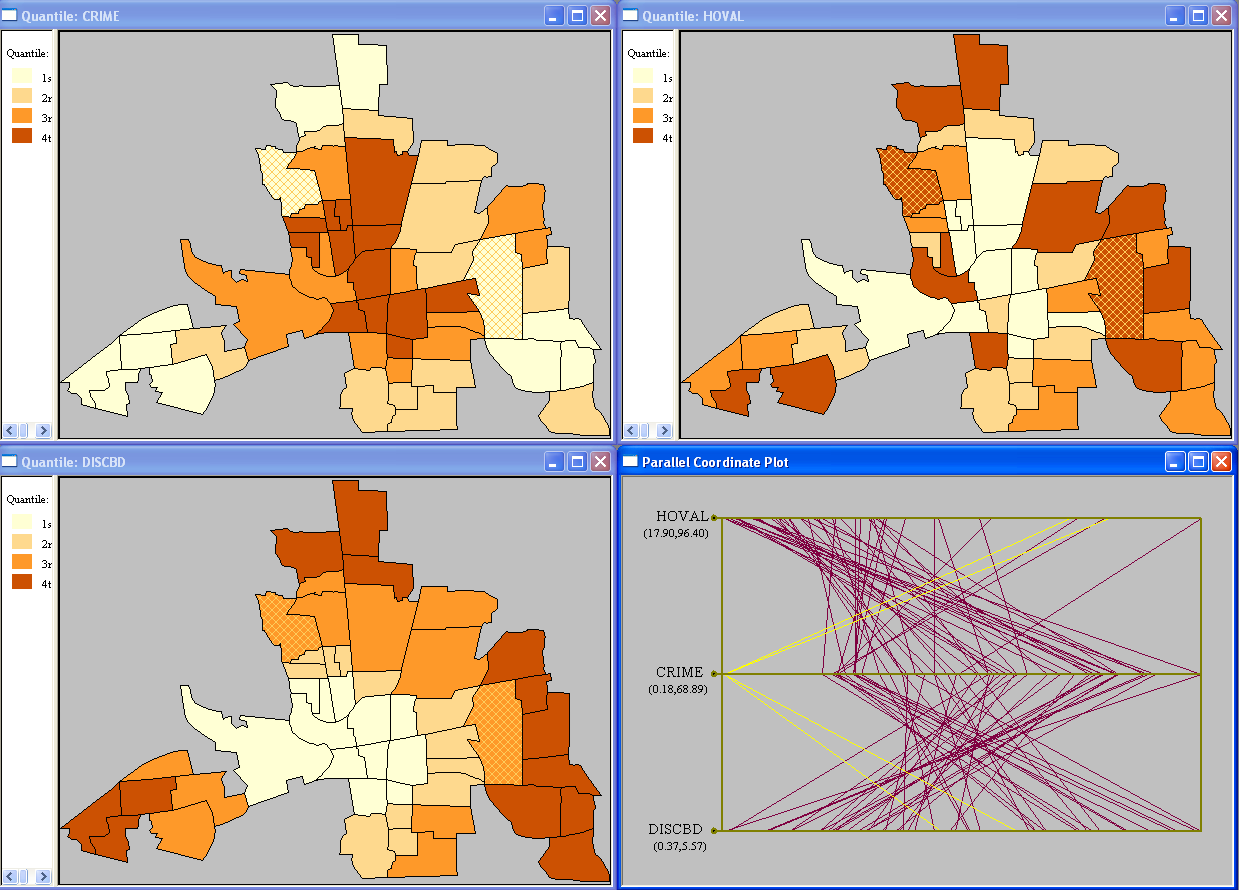
\includegraphics[width=.85\linewidth]{brushpcpgeoda.png}
  \end{center}
 \end{frame} 

\begin{frame}
	\frametitle{Brushing in 3-D}
 \begin{center}
 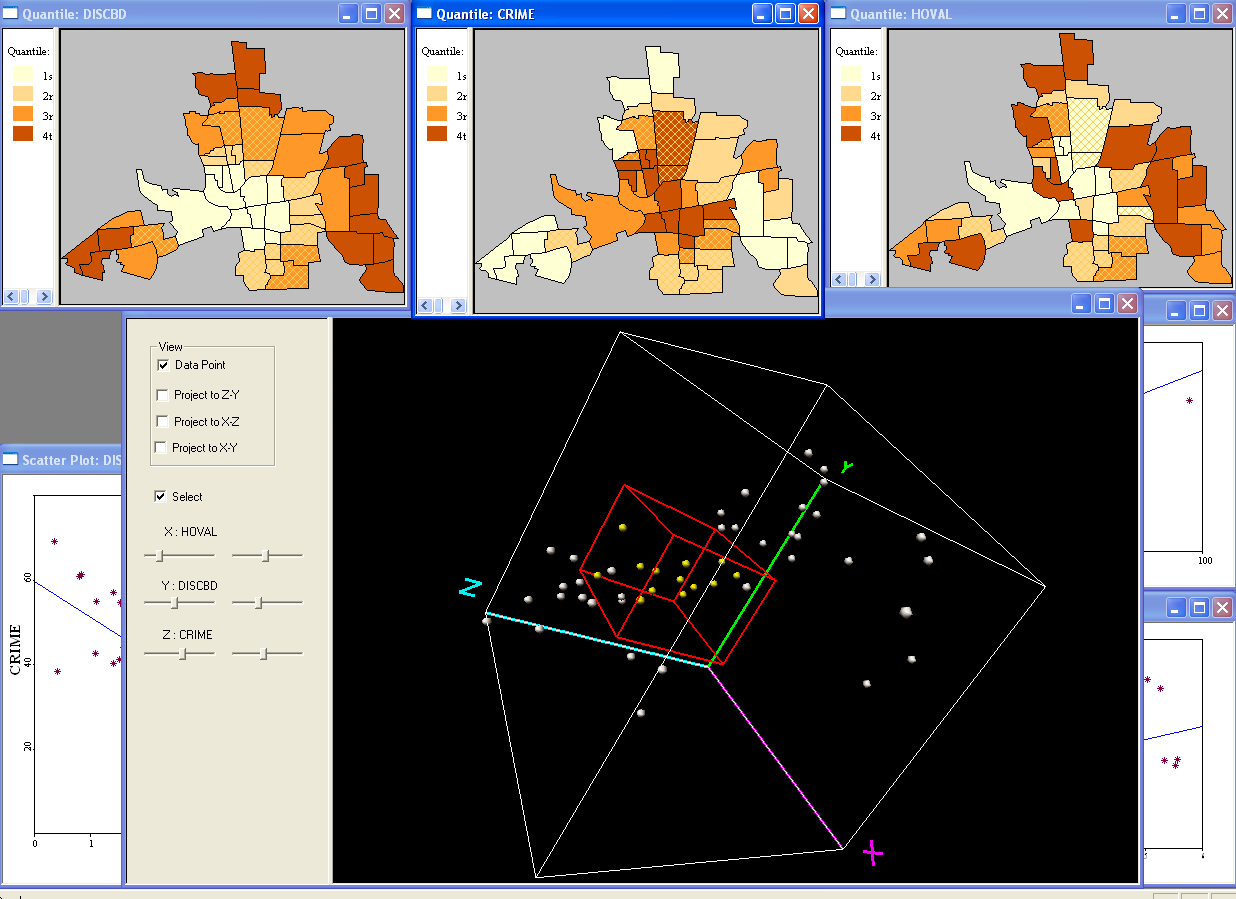
\includegraphics[width=.85\linewidth]{select3d.png}
  \end{center}
 \end{frame}
\end{document}
